\textbf{Date:} May 28th 2014\\\textbf{Duration:} 12-16\\\textbf{Group
members:} Henrik, Jakob, Jesper

\subsection{Goal}

Due to the troubles we had with distinguishing intersections in order to
navigate, we figured it may be worth our while to scrap the line
follower approach entirely, and try navigating through the tacho
counter. This will be quick to implement, and if it's able to stay on
track, we will have saved a lot of time.\\And so, our goal for today is
to explore the possibility of using a tacho counter, whilst trying to
improve the line follower.
\begin{figure}[hbt]
  \centering
  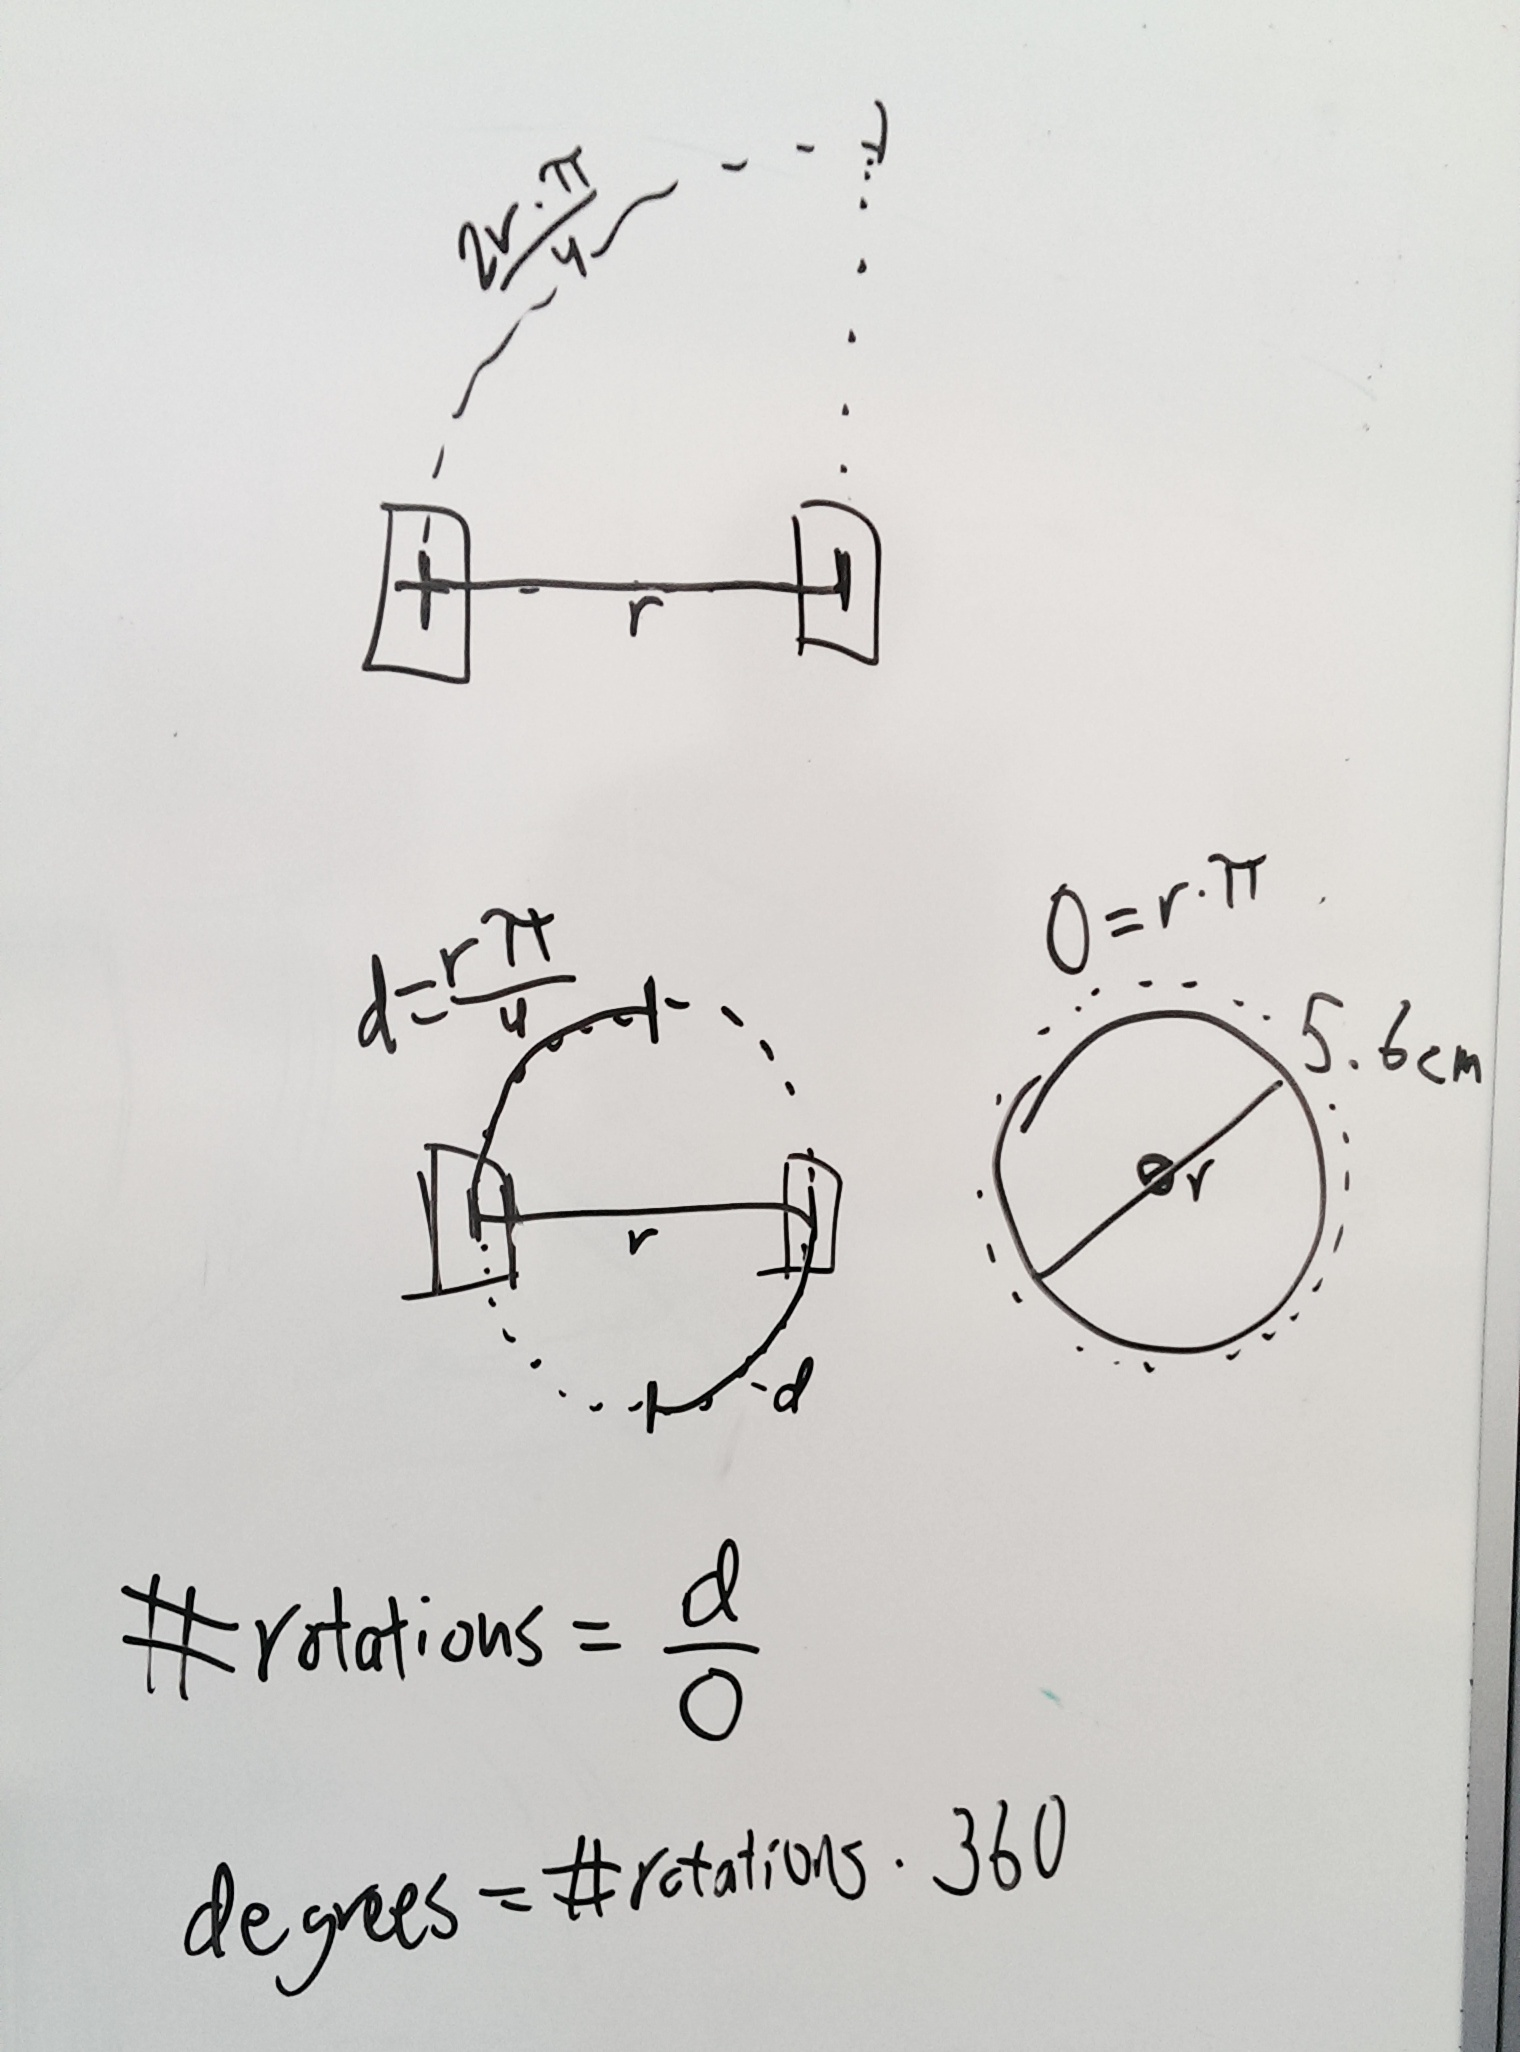
\includegraphics[scale=0.1]{../experiments/images/maths.jpg}
\caption{Top: first approach to turning. Middle: rotating on the spot, better approach}
\end{figure}

Number of degrees required to move x centimeters forward:
$$\#degrees = 360\frac{distanceInCm}{wheelCircumference} = \frac{360\cdot distanceInCm}{wheelDiameter \cdot \pi}$$
Number of degrees wheel turning required to rotate the vehiccle 90 degrees:
$$\#degrees = 360 \cdot \frac{vehicleWidth\cdot 2\cdot \pi/4}{wheelDiameter \cdot \pi}$$
\\
\\
\begin{lstlisting}[language=java]
  public static void forward(float distance){ 
    int degrees = (int)(360*distance / (wheelSize * Math.PI));
    Motor.B.rotate(degrees, true);
    Motor.C.rotate(degrees);
  }

  public static void right(){
    double degrees = 360*((width*2 * Math.PI)/4)
      /(wheelSize * Math.PI);  //wheel rotations required for a 90 degree turn of the vehicle
    degrees = degrees * 1.05f; //taking slight inaccuracies into account
    Motor.B.rotate((int)degrees/2, true);
    Motor.C.rotate((int)-degrees/2);
    }
\end{lstlisting}

Using these two methods, and a similar method for left(), and measuring
the track in centimeters, we were able to get the vehicle to cover the
whole track in a short time. After the first couple of turns it became
quite inaccurate though, and we quickly saw the downside of driving
using only the tacho counter. In addition to that, the vehicle we have
is rather flexible due to a shoddy build, and this makes the wheels
slide around, reducing the accuracy of the vehicle.

While the tacho counter method was being developed, a line follower was
being written and tested simultaneously. We tried to implement a PID
controller from previous weeks to make the vehicle better at line
following, but it later occurred to us that since there are no difficult
curves on the track, this is unnecessary. Instead we implemented a
proportional controller, and the results were promising. The vehicle
could follow a straight line without issues.

\subsection{Conclusion}

Implementing a tacho navigator would require us to rebuild the vehicle
and spend a lot of time tweaking parameters in order for it to not lose
track of its position, and even then it will have no way of correcting
its course. Therefore it is not a feasible solution.\\We will proceed
with the newly implemented P controller, and use that for line
following.
